\chapter{Xây dựng hệ thống phân loại tự động}
\paragraph{Giới thiệu} Qua các chương trước, chúng em đã trình bày các cơ sở lý thuyết gồm OWL 2, SWRL, đề ra các thiết kế cho hệ thống và thiết kế một ontology sử dụng cho việc phân loại. Trong chương này, chúng em sẽ trình bày lại quá trình xây dựng hệ thống phân loại dựa trên các thiết kế ở chương trước.
\section{UI của ứng dụng - OWLEditorUI}
\subsection{Giới thiệu OWLEditorUI}
Lớp này được mở rộng từ lớp \textbf{UI} của Vaadin - chức năng cơ bản của \textbf{UI} là nơi khởi tạo mọi thành phần giao diện và trình bày nó dưới dạng HTML trên web page, OWLEditorUI mở rộng các chức năng trên như sau:
\begin{itemize}
\item Chứa EntryView, MainView (các View này chứa tất cả thành phần giao diện của hệ thống)
\item Cập nhật và cài đặt MainView khi ontology được nạp vào EntryView.
\item Cập nhật trạng thái khi người dùng refresh trang.
\item Nạp (inject) OWLEditorKit và cung cấp nó qua phương thức tĩnh (static).
\item Nạp EventBus và cung cấp qua các phương thức tĩnh.
\item Nạp HttpSession và cung cấp qua phương thức tĩnh .
\end{itemize}
\subsection{Chi tiết các chức năng của OWLEditorUI}
Trước khi đi vào chi tiết các chức năng trên, chúng em muốn giới thiệu khái quát về cách thức hoạt động của Spring Boot \cite{springboot}, các Annotation đáng chú ý được sử dụng trong việc xây dựng hệ thống.
\\
\textbf{Spring Boot} : Khi chương trình khởi động - nghĩa là khi chương trình được nạp vào một hệ thống Servlet như Tomcat, Jetty thì điểm xuất phát đầu tiên của chương trình sẽ từ đối tượng sau:
\begin{verbatim}
@SpringBootApplication public class OWLEditorApplication {
    public static void main(String[] args) {
       SpringApplication.run(OWLEditorApplication.class, args); }
}
\end{verbatim} 
@SpringBootApplication là một tên thay thế cho 3 annotation gồm \textbf{@Configuration}, \textbf{@EnableAutoConfiguration} và \textbf{@ComponentScan} (sẽ được giới thiệu ở dưới), mục tiêu của đối tượng này là khởi động ứng dụng, duyệt hết trong package hiện hành tới package con để tìm các Component Bean cần thiết để khởi tạo và thực thi các Bean đó. Cụ thể ở đây, nó sẽ quét vào tìm thấy \textbf{OWLEditorUI} được đánh dấu bằng \textbf{@VaadinUI} và chạy theo cấu hình có săn được định nghĩa trong Spring 4 Vaadin \cite{spring4vaadin}. Từ đây mọi thứ sẽ diễn ra trong \textbf{OWLEditorUI}. Ý nghĩa của các Annotation:
\begin{itemize}	
\item \textbf{@VaadinUI} Là annotation của Spring 4 Vaadin \cite{spring4vaadin} khai báo một lớp là một Bean và là một Vaadin \textbf{UI} cho hệ thống Spring Boot.
\item \textbf{@VaadinComponent} Là annotation của Spring 4 Vaadin, tương tự annotation @Component của Spring Framework: khai báo đây là một Bean cơ bản nhất cho hệ thống Spring Boot.
\item \textbf{@Repository} Là annotation của Spring Framework, khai báo một đối tượng là một Bean với tính chất là nơi để lấy và khai thác dữ liệu, OWLEditorKit được khai báo bằng annotation này.
\item \textbf{@Autowired} Là annotaion của Spring Framework, dùng nạp tự động các Bean đã được khai báo (bằng các annotation như @VaadinComponent, @Component, @Repository, ...) vào hệ thống, cụ thể chúng em dùng các đối tượng này để nạp OWLEditorKit, HttpSession và OWLEditorEventBus vào OWLEditorUI.
\item \textbf{@Theme} Là annotation của Vaadin dùng để nạp thành phần tùy chỉnh CSS cho toàn bộ giao diện của hệ thống.
\item \textbf{@EnableAutoConfiguration} Là annotation của Spring Boot, bật tính năng cấu hình tự động (mọi cấu hình về DataBase, Base Url,... sẽ ở trạng thái mặc định).
\item \textbf{@ComponentScan} Là annotation của Spring, tự động quét và tìm các Bean từ package hiện hành và khởi tạo chúng.
\item \textbf{@Nonnull} Là annotation từ JSR-305, đảm bảo tham số nhập vào không được null, nếu null tự động throw NullPointerException.
\end{itemize}
\subsubsection{Sử dụng OWLEditorKit trong OWLEditorUI}
Như đã nói sơ qua, thì \textbf{OWLEditorKit} được định nghĩa là một Bean của hệ thống nên khi khởi động nó sẽ được tạo ra nhờ tính năng duyệt Bean vừa giới thiệu. Trong OWLEditorUI, chúng ta sẽ nạp (inject) nó vào OWLEditorUI và tạo một phương thức tĩnh để có thể sử dụng từ các thành phần giao diện như sau:
\begin{verbatim}
@Autowired OWLEditorKit eKit; 
public static OWLEditorKit getOWLEditorKit() {
  ((OWLEditorKit) UI.getCurrent()).eKit; }
\end{verbatim}
Lưu ý: \textit{UI.getCurrent()} là một hàm tiện ích của Vaadin nhằm trả về UI đang chạy hiện hành, trong hệ thống mà chúng em xây dựng chỉ có duy nhất một UI là OWLEditorUI nên sẽ ép kiểu trực tiếp, trong trường hợp có nhiều UI cần lưu ý vấn đề kiểm tra loại UI. Trong source code \cite{owleditorSrc}, chúng em chỉ khai báo Annotation @Repository cho lớp \textit{OWLEditorKitImpl} vậy tại sao @Autowired lại biết mà khởi tạo được ? Câu trả lời là hệ thống sẽ quét và tìm đến các lớp áp dụng interface OWLEditorKit mà có Annotation khai báo để khởi tạo. Để đơn giản ở đây chúng em sẽ dùng hàm khởi tạo mặc định trong OWLEditorKitImpl, ngoài ra còn rất nhiều cách thức @Autowired (hoặc inject) khác có thể tham khảo ở \cite{springboot}.
\subsubsection{Sử dụng OWLEditorEventBus trong OWLEditorUI}
Trong thiết kế chúng em sẽ sử dụng \textit{một} EventBus để xử lý sự kiện cho hệ thống, vì vậy sẽ dễ dàng hơn nếu nó được khởi tạo một lần trong OWLEditorUI và cung cấp dưới dạng phương thức tĩnh. Đầu tiên là cấu trúc của một lớp dùng chứa EventBus thật sự và cách tạo ra các hàm tĩnh.
\begin{verbatim}
@VaadinComponent public class OWLEditorEventBus {
  private final EventBus realEventBus = new EventBus(this); //từ Guava API
  public static void post(@Nonnull final Object event) {
    OWLEditorUI.getGuavaEventBus().realEventBus.post(event);  }
  public static void register(@Nonnull final Object obj) { ... } ...
}
// Trong OWLEditorUI
@Autowired OWLEditorEventBus eventBus;
public static OWLEditorEventBus getGuavaEventBus() {
  ((OWLEditorKit) UI.getCurrent()).eventBus; }
\end{verbatim}
Vậy để sử dụng Guava EventBus trong OWLEditorUI, chỉ cần gọi \textit{OWLEditorUI. getGuavaEventBus} hoặc đơn giản hơn \textit{OWLEditorEventBus. <tên phương thức>}.
\subsubsection{Sử dụng HttpSession trong OWLEditorUI}
Tương tự 2 thành phần trên, HttpSession cũng là một Bean có sẵn của Spring nên chúng ta có thể nạp vào OWLEditorUI và sử dụng như sau:
\begin{verbatim}
@Autowired HttpSession httpSession;
public static HttpSession getHttpSession() {
 return ((OWLEditorUI) getCurrent()).httpSession; }
\end{verbatim}
\subsubsection{Cập nhật trạng thái giữa EntryView và MainView}
\begin{figure}[h!]
	\centering
	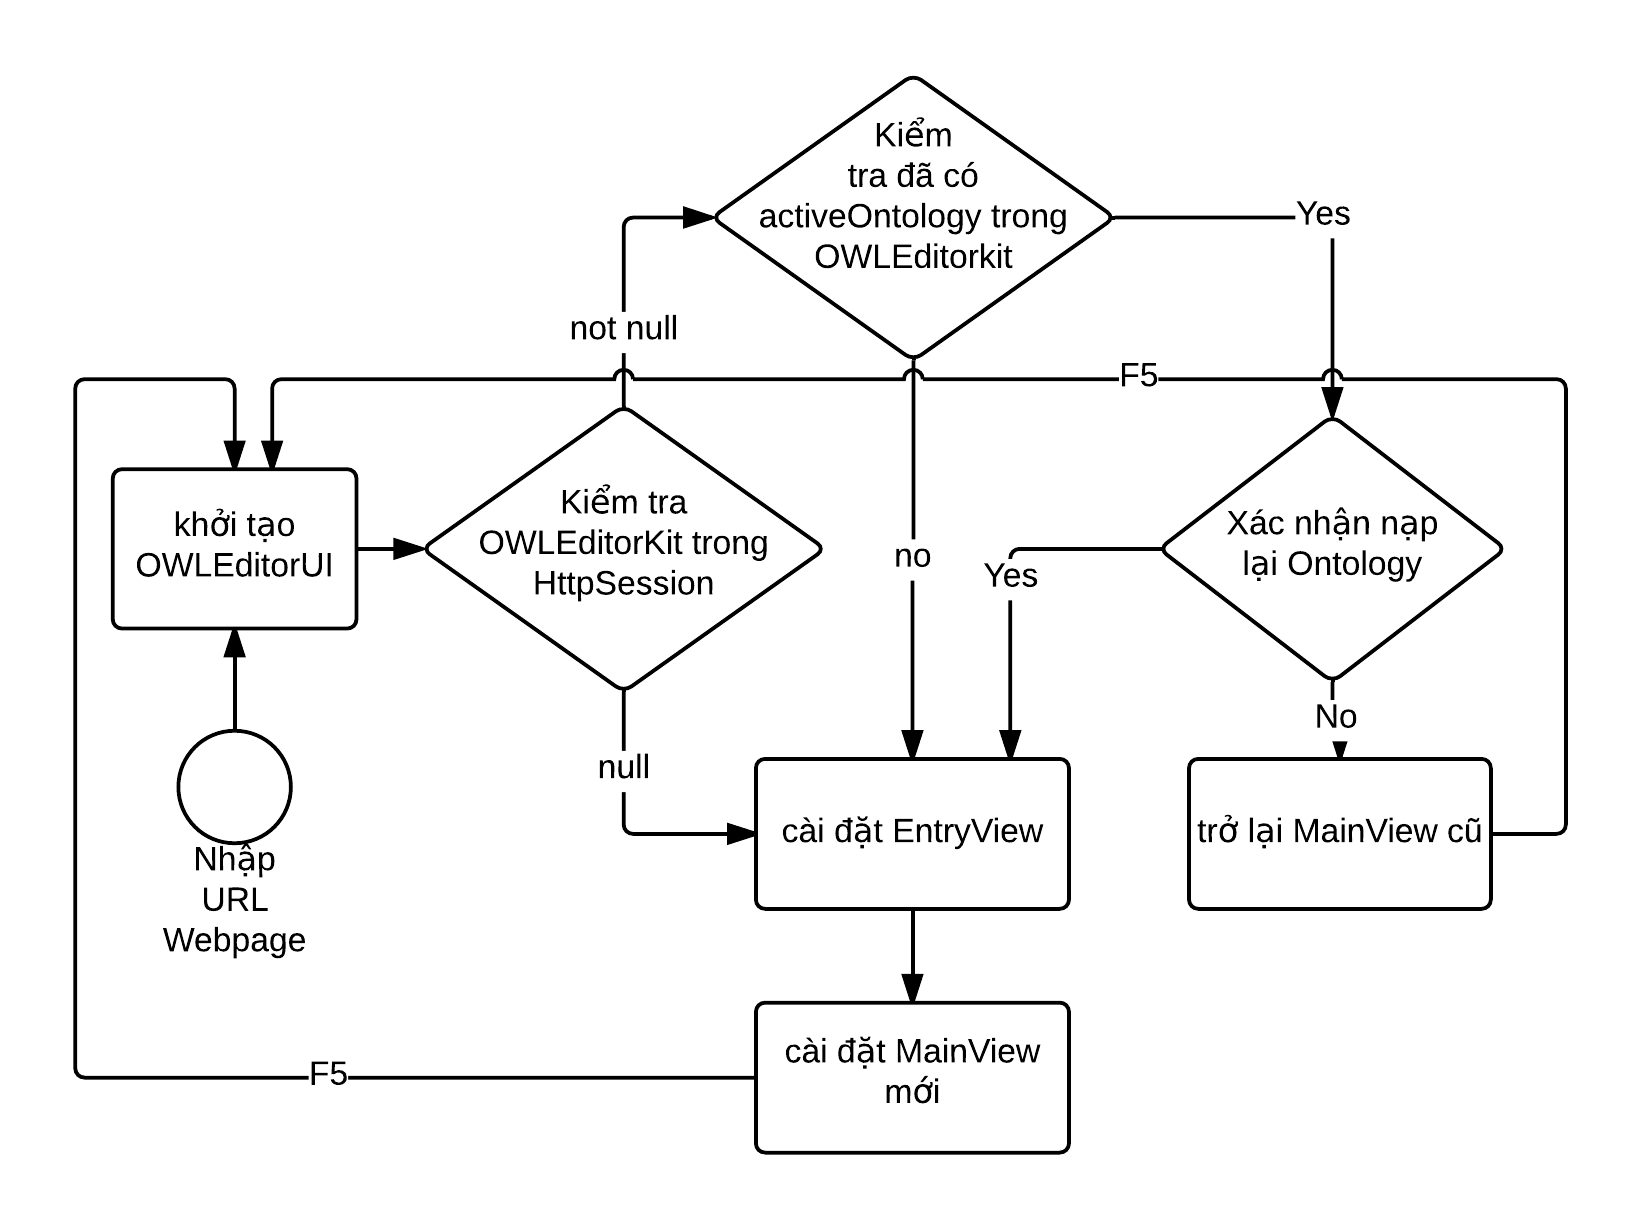
\includegraphics[width=150mm]{Figures/owleditorui_flowchart.png}
	\caption{Vòng đời của các view trong OWLEditorUI \label{overflow}}
\end{figure}
Mỗi lần chúng ta vào trang url của ứng dụng hay refresh thì vòng đời của các View sẽ diễn ra như trong hình 4.1. Việc kiểm tra các điều kiện đều nằm trong phương thức \textbf{updateContent} của OWLEditorUI.
\textbf{Tóm lại} OWLEditorUI là nơi sẽ cung cấp các thành phần lõi của hệ thống như OWLEditorKit, EventBus và HttpSession. Tiếp theo, chúng em sẽ trình bày cách xây dựng các View và thành phần của chúng.
\section{Xây dựng EntryView}
Như được thiết kế thì giao diện của EntryView tương đối đơn giản, chỉ có 1 panel chứa các input để nạp ontology theo 3 tùy chọn:
\begin{enumerate}
\item Nạp ontology qua URL. URL này bắt buộc phải là một tài liệu được định dạng theo tiêu chuẩn OWL 2 (RDF/XML, OWL/XML, FunctionalSyntax/XML,...).
\item Upload một tập tin chứa tài liệu Ontology và nạp tài liệu ontology này vào.
\item Tạo mới một tài liệu ontology.
\end{enumerate}
{\let\thefootnote\relax\footnotetext{
	\begin{enumerate}
		\item \textit{HorizontalLayout} các UI Component được sắp xếp theo chiều ngang, từ trái qua phải.
		\item \textit{VerticalLayout} các UI Component được sắp xếp theo chiều dọc, từ trên xuống.
		\item \textit{AbsoluteLayout} các UI Component được sắp xếp theo đúng vị trí tọa độ được khai báo.
		\item \textit{CssLayout} các UI Component được sắp xếp theo định nghĩa từ các file css tương ứng.
	\end{enumerate}}
}
\begin{figure}[h!]
	\centering
	\frame{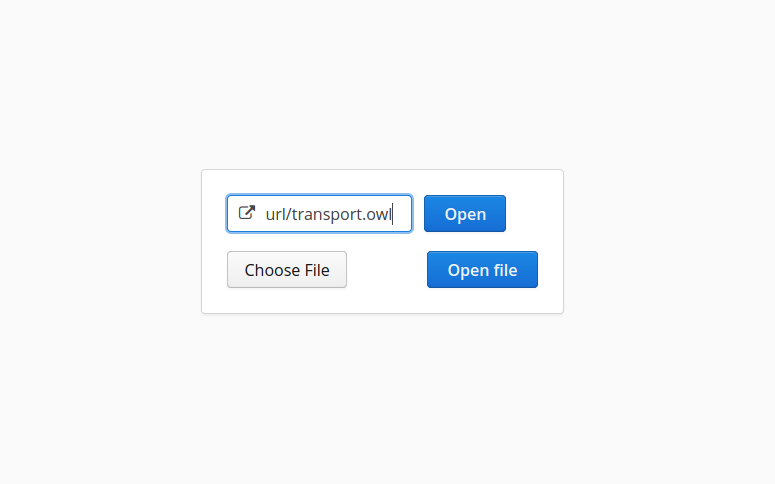
\includegraphics[width=145mm]{Figures/owleditor_entryview.png}}
	\caption{EntryView đã xây dựng\label{overflow}}
\end{figure}
Giao diện EntryView được mở rộng từ layout \textit{VerticalLayout}\textsuperscript{*}, để chứa panel ở giữa - panel này cũng là một \textit{VerticalLayout} tập hợp mỗi dòng là một \textit{HorizontalLayout}, mỗi \textit{HorizontalLayout} này sẽ chứa một \textit{TextField} và một \textit{Button} hoặc một \textit{UploadField} và một \textit{Button} (Hình 4.2) - tất cả các thành phần vừa nêu đều được cung cấp bởi Vaadin. Nhờ vậy, việc xây dựng giao diện khá dễ dàng, chẳng hạn để đặt vị trí trung tâm cho panel trong hình chỉ cần sử dụng dòng code sau :
\begin{verbatim}
setComponentAlignment(entriesPanel, Alignment.MIDDLE_CENTER);
\end{verbatim}
Sau khi click "Open", nếu URL chứa tài liệu hợp lệ thì nó sẽ được nạp vào trong OWLEditorKit, nếu đây là lần đầu OWLEditorKit được sử dụng và chưa được lưu trong HttpSession thì lưu nó vào Session và cuối cùng là chuyển giao diện qua \textit{MainView} (Hình 4.1). Quá trình tương tự cũng xảy ra khi nạp tài liệu từ tập tin upload và tạo mới tài liệu, riêng việc tạo tài liệu thì chúng ta có thể tùy chọn đặt 1 IRI cho nó trong TextField ở dòng cuối. Upload file cũng là một plugin được cung cấp qua \cite{vaadindirectory}, nên việc sử dụng cũng rất đơn giản.
\begin{verbatim}
UploadField uf = new UploadField();
// code bên trong "Open" Button ClickListener
File file = (File) uf.getValue();
OWLEditorUI.getEditorKit() // Nạp ontology vào trong OWLEditorKit
           .loadOntologyFromOntologyDocument(IRI.create(file));
OWLEditorUI.getHttpSession() // lưu OWLEditorKit trong Session
           .setAttribute("OWLEditorKit", OWLEditorUI.getEditorKit());
// Đặt giao diện là MainView 
UI.getCurrent().setContent(new MainView());                    
\end{verbatim}

\section{Xây dựng MainView}
Trong thiết kế hệ thống, \textit{MainView} sẽ là nơi chứa tất cả các Tab của ứng dụng, các Tab này được xây dựng dựa trên thành phần \textit{TabSheet} của Vaadin, mỗi Tab đều có thể là bất cứ thành phần giao diện nào của Vaadin (UIComponent và Layout của Vaadin đều có chung Interface \textit{Component}). Do vậy, nội dung của MainView khá đơn giản:
\begin{verbatim}
public class MainView extends HorizontalLayout {
  final TabSheet root = new TabSheet();
  public MainView() {
    root.addTab(new ClassesSheet(), "Classes");
    addComponent(root); // Thêm TabSheet vào layout của MainView;
    ...}
} 
\end{verbatim}
\subsection{Xây dựng Tab Sheet để mô tả lớp, thuộc tính đối tượng/dữ liệu và cá thể}
Do bố cục phần lớn các thành phần trong các Tab này cũng tương đối giống nhau, nên chúng em sẽ dùng Tab Classes để trình bày chi tiết, với những Tab còn lại chúng đều có cách xây dựng tương tự.
\subsubsection{Sheet}
Đây là lớp chúng em dùng để tổ chức các thành phần giao diện dành để tương tác với các lớp trong OWL 2 Ontology.
\begin{figure}[h!]
	\centering
	\frame{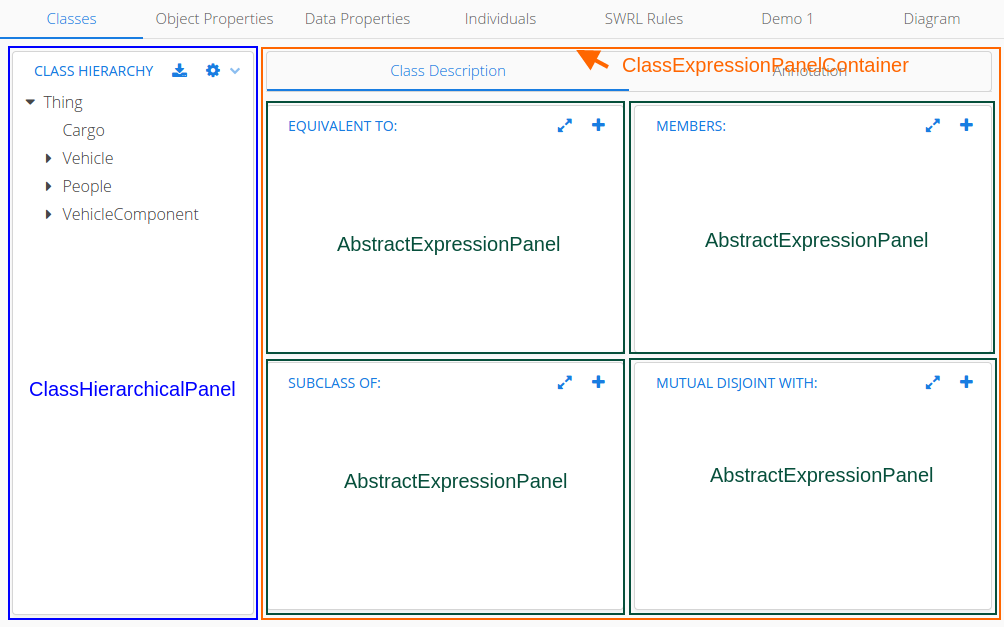
\includegraphics[width=155mm]{Figures/owleditor_mainview.png}}
	\caption{ClassSheet(Tab dành cho lớp) đã xây dựng\label{overflow}}
\end{figure}
{\let\thefootnote\relax\footnotetext{
		Lưu ý:  \textit{ClassHierarchicalPanel}, \textit{ObjectPropertyHierachicalPanel} và \textit{DataPropertyHierarchicalPanel} đều kế thừa từ \textit{AbstractHierarchyPanel}.
}}
ClassSheet cũng là một Layout gồm 2 thành phần con là ClassHierarchicalPanel và ClassExpressionPanelsContainer, đây là nơi bắt sự kiện lựa chọn lớp trên cấu trúc cây của ClassHierarchicalPanel để gán lớp này vào làm dữ liệu cho các panel con bên phải (Hình 4.3).
\subsubsection{AbstractHierarchyPanel}
Ở bên trái là một Panel gọi là \textit{ClassHierarchicalPanel} (Hình 4.3) mở rộng từ \textit{AbstractHierarchyPanel} \textsuperscript{*} được chúng em xây dựng với mục tiêu là biểu diễn các lớp trong OWL 2 Ontology, và cho phép thực hiện các thao tác thêm lớp con, lớp cùng họ (sibling) và xóa lớp bằng cách click phải vào bất kì node nào trên cây. Ở góc phải bên trên của panel này, với kí hiệu bánh răng với chức năng thêm xóa tương tự, ngoài ra còn có tính năng bật reasoner cho hệ thống. Kế bên kí hiệu bánh răng, là một kí hiệu tải xuống, khi click sẽ lưu lại trạng thái ontology hiện hành và tải xuống dưới định dạng OWL/XML.
\\
Bên trong \textit{ClassHierarchicalPanel} có thành phần \textit{Tree} đây chính là thành phần sẽ liên kết với dữ liệu từ các \textit{HiearchicalContainer} được giới thiệu trong mục tổ chức dữ liệu ở chương trước, ở đây cụ thể nó sẽ liên kết với các \textit{ClassHierarchicalContainer} - chứa các lớp trong ontology với cấu trúc phân cấp. Nếu đúng như trong thiết kế thì chúng em sẽ sử dụng EventBus để xử lý các sự kiện thêm/xóa lớp ở đây, tuy nhiên sau khi xây dựng xong chúng em gặp phải vấn đề về con-current event - nghĩa là khi thực hiện thao tác thêm/xóa sẽ có 2 event giống nhau được tạo ra và truyền lên EventBus. Do vẫn chưa tìm được nguyên nhân chính xác, nên chúng em đã quay về với thiết kế truyền thống của Java là tạo một interface \textit{OWLEntityActionHandler} vào áp dụng nó vào thành phần \textit{Tree} (Hình 4.4).
\begin{figure}[h!]
	\centering
	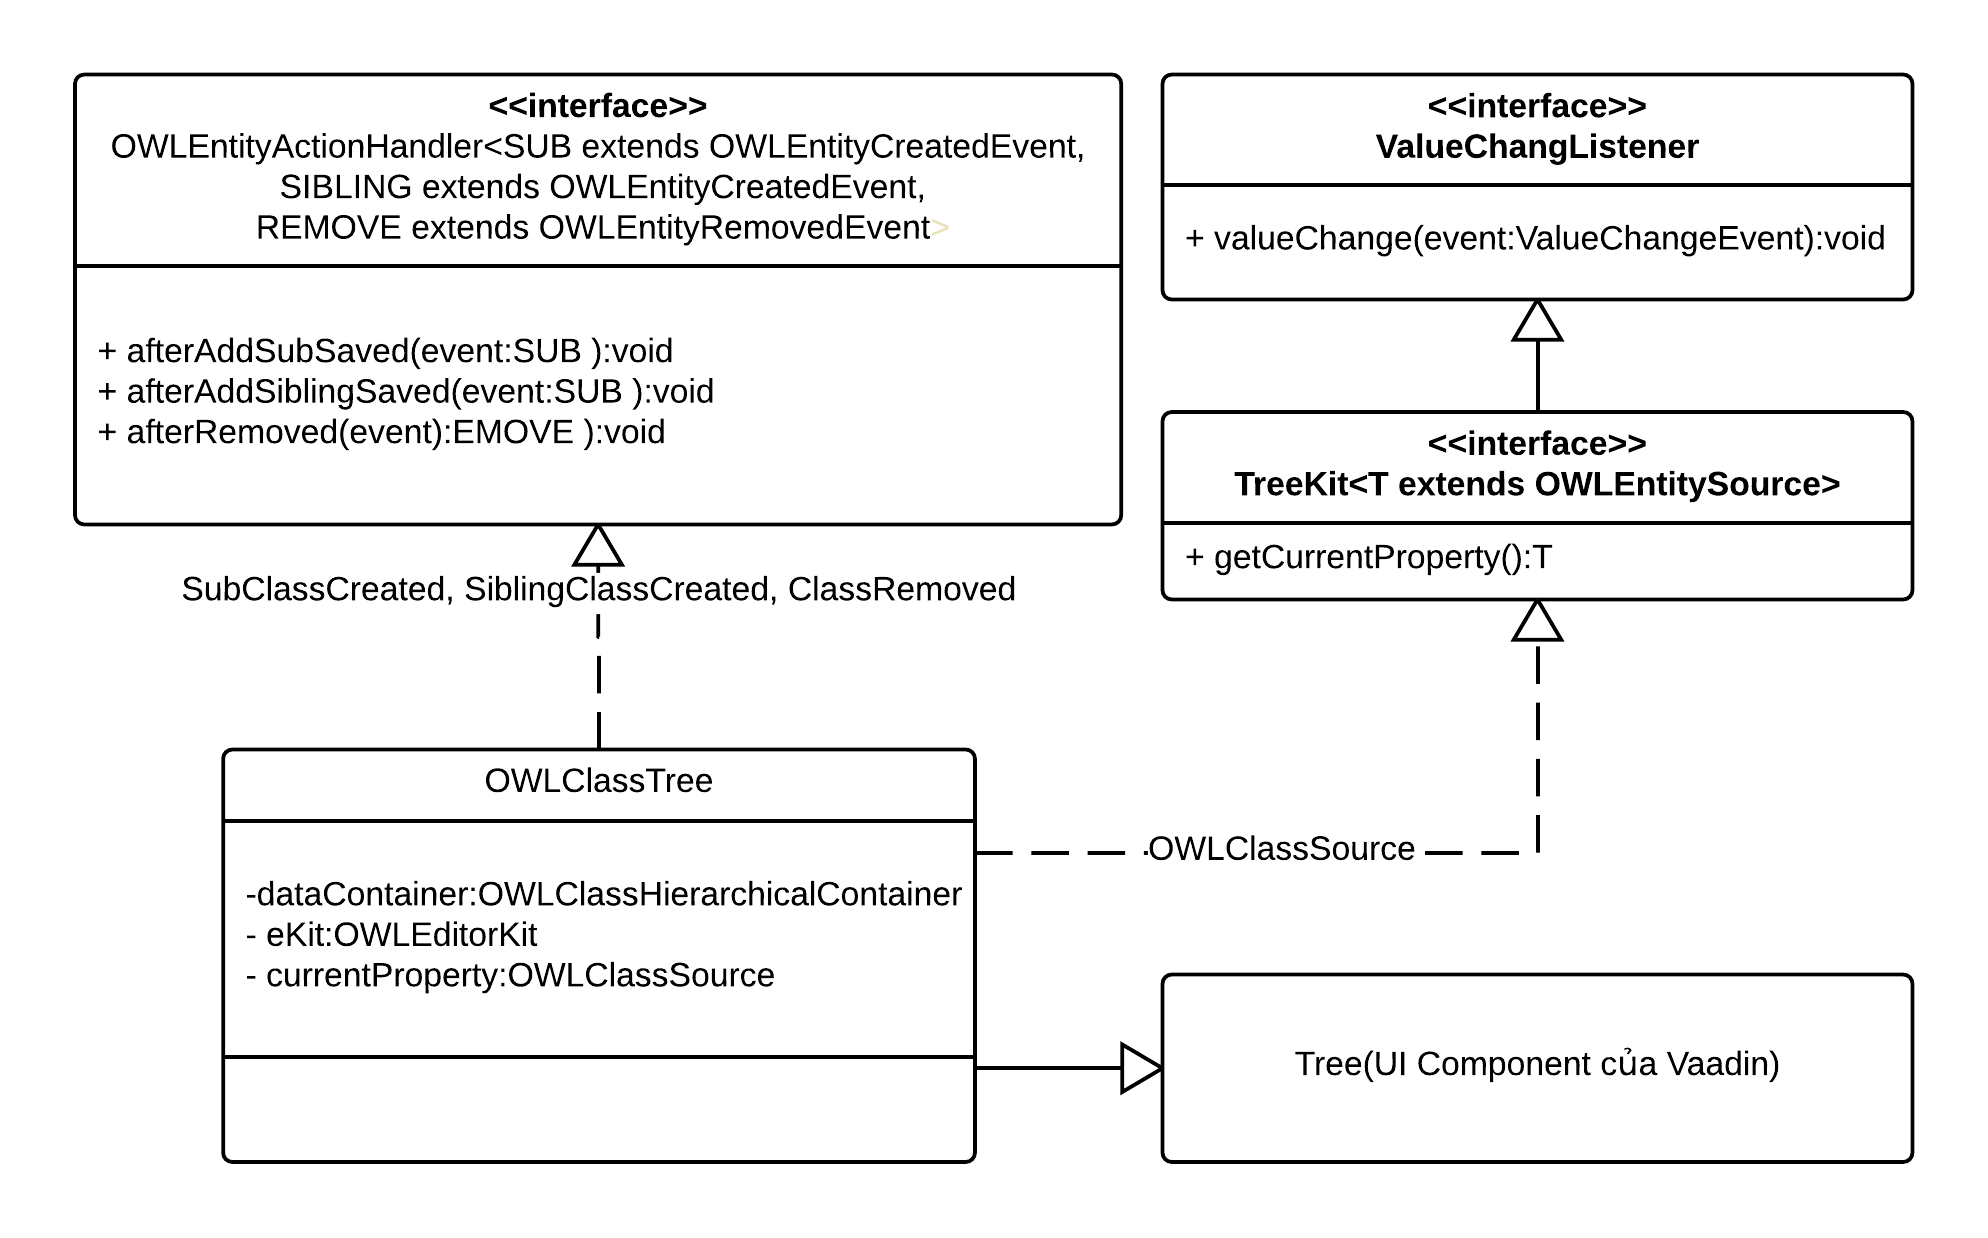
\includegraphics[width=155mm]{Figures/uml_owlclasstree.png}
	\caption{Class Diagram của OWLClassTree các interface của nó \label{overflow}}
\end{figure}
\begin{figure}[h!]
	\centering
	\frame{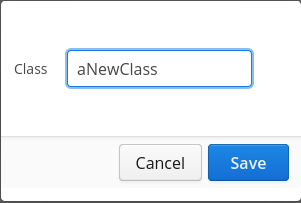
\includegraphics[width=80mm]{Figures/owleditor_addentitywd.png}}
	\caption{Cửa sổ thêm thực thể \textit{lớp} trong ClassSheet \label{overflow}}
\end{figure}
Thao tác thêm mới cửa sổ dùng để nhập tên lớp mới (Hình 4.5), cửa sổ này là lớp \textit{buildAddOWLClassWindow} mở rộng từ \textit{AbstractAddOWLObjectWindow} (Hình 4.6). Đối tượng này phải biết OWLEntityActionHandler (là OWLClassTree hình 4.4) để khi chọn save nó sẽ sử dụng action handler này để áp dụng các thay đổi lên ontology và lên giao diện cây sẽ tự động thêm node con, hay node cùng họ (Sibling) - tương ứng với tùy chọn Sub Class hay Sibling Class. Chính vì thế nên hàm khởi tạo của lớp này sẽ buộc phải có tham số \textit{OWLEntityActionHandler}, để sử dụng khi click save (phần note Hình 4.6).
\begin{figure}[h!]
	\centering
	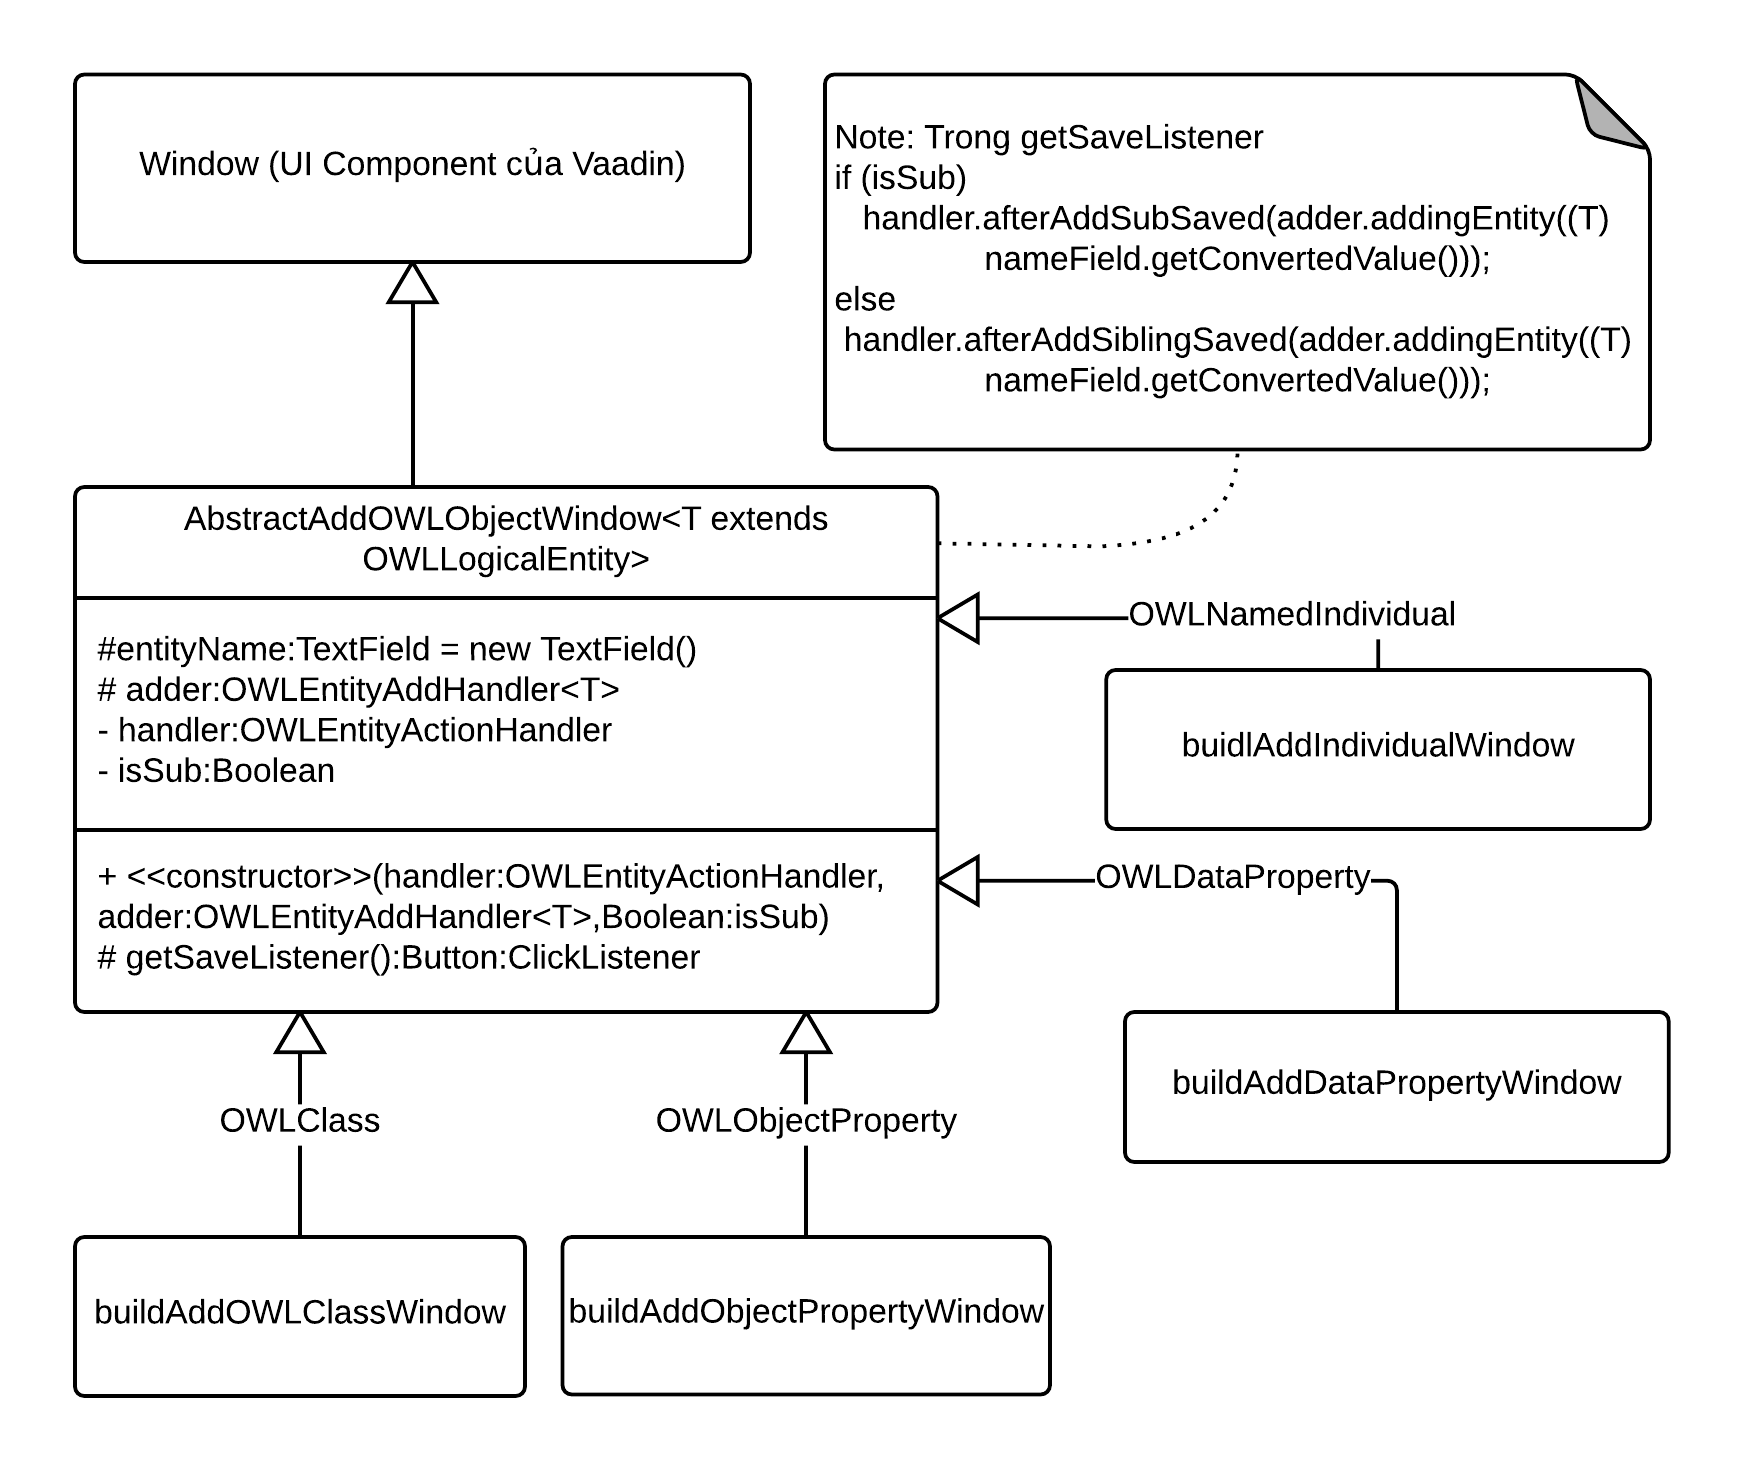
\includegraphics[width=155mm]{Figures/uml_addowlobjectwindow.png}
	\caption{Class Diagram của  AbstractAddOWLObjectWindow\label{overflow}}
\end{figure}
Ngoài interface \textit{OWLEntityActionHandler}, thì trong hình chúng ta còn thấy một đối tượng là \textit{OWLEntityAddHandler} (hàm khởi tạo và phần note hình 4.6). Đây là một Interface hỗ trợ cho việc tạo ra các sự kiện liên quan thêm các thực thể \textit{OWLEntityCreatedEvent} (giới thiệu trong chương trước). Vì trong lớp Abstract, chúng ta chưa biết phải trả về loại sự kiện tạo lớp hay thuộc tính hay cá thể, nên Interface này sẽ giúp chúng ta nạp vào loại sự kiện phù hợp. Ví dụ chúng ta muốn tạo một cửa sổ con để khai báo mới một thuộc tính dữ liệu con:
\begin{verbatim}
Window w = new AbstractAddOWLObjectWindo<OWLDataProperty>(
 actionHandler,
 newDataPropery -> new SiblingClassCreated(newDataPropery, 
                   owlClassTree.getSelectedProperty),
 true);// True là tạo thực thể con
\end{verbatim}
Ngoài ra chúng ta còn tận dụng được một đặc điểm mới của ngôn ngữ Java 8 là Lambda Expression (obj -> function). Rất nhiều Interface dạng này được tạo ra nhằm giảm thiểu việc phải code lại nhiều lần với cùng một mục đích là tạo ra các sự kiện. Đây cũng chính là lý do vì sao các sự kiện lại được thiết kế để khai thác tính đa hình của hướng đối tượng.
\\
Như đã trình bày trong chương 3, các thành phần mở rộng từ \textit{Tree} của Vaadin có khả năng liên kết với các dữ liệu dạng phân cấp hay cụ thể chúng em sử dụng OWLClassHierachicalContainer cho OWLClassTree trong trường hợp này. Ngoài ra, OWLClassHierachicalContainer còn được sử dụng để lắng nghe mọi thay đổi bên trong ontology qua:
\begin{verbatim}
public OWLClassTree() {
  editorKit.getModelManager().addOntologyChangeListener(
  changes -> { for (OWLOntologyChange chg :changes) { 
   chg.accept(dataContainer.getOWLOntologyChangeListener());}
});       
\end{verbatim}
Nhờ vậy, khi dữ liệu bên trong Container thay đổi, nó sẽ thông báo đến các thành phần giao diện mà nó liên kết để cập nhật thay đổi mà không code để thực hiện các thay đổi trên giao diện.
\subsubsection{AbstractExpressionPanel}
Nằm ở bên phải của Tab ClassSheet là một container chứa nhiều panel nhỏ khác (Hình 4.3), mỗi panel nhỏ này đóng vai trò là nơi tương tác với từng loai phát biểu liên quan đến lớp đang được chọn trên cấu trúc cây. Khi một lớp được chọn, trong ClassSheet sẽ gọi đến phương thức sau đây của \textit{ClassExpressionPanelsContainer}.
\begin{verbatim}
setPropertyDataSource(Property newDataSource) {
  equivPanel.setPropertyDataSource(newDataSource);
  ...}
\end{verbatim}

Phương thức này sẽ gọi một phương thức tương tự trong các panel nhỏ bên trong đặt \textit{Property} cho chúng - Property này chỉnh là Data Model dạng Property đã thiết kế trong chương 3. Các panel này tuy nhiều nhưng thật ra chúng em xây dựng chúng đều trên một lớp Abstract gọi là \textit{AbstractExpressionPanel}.
\begin{figure}[h!]
	\centering
	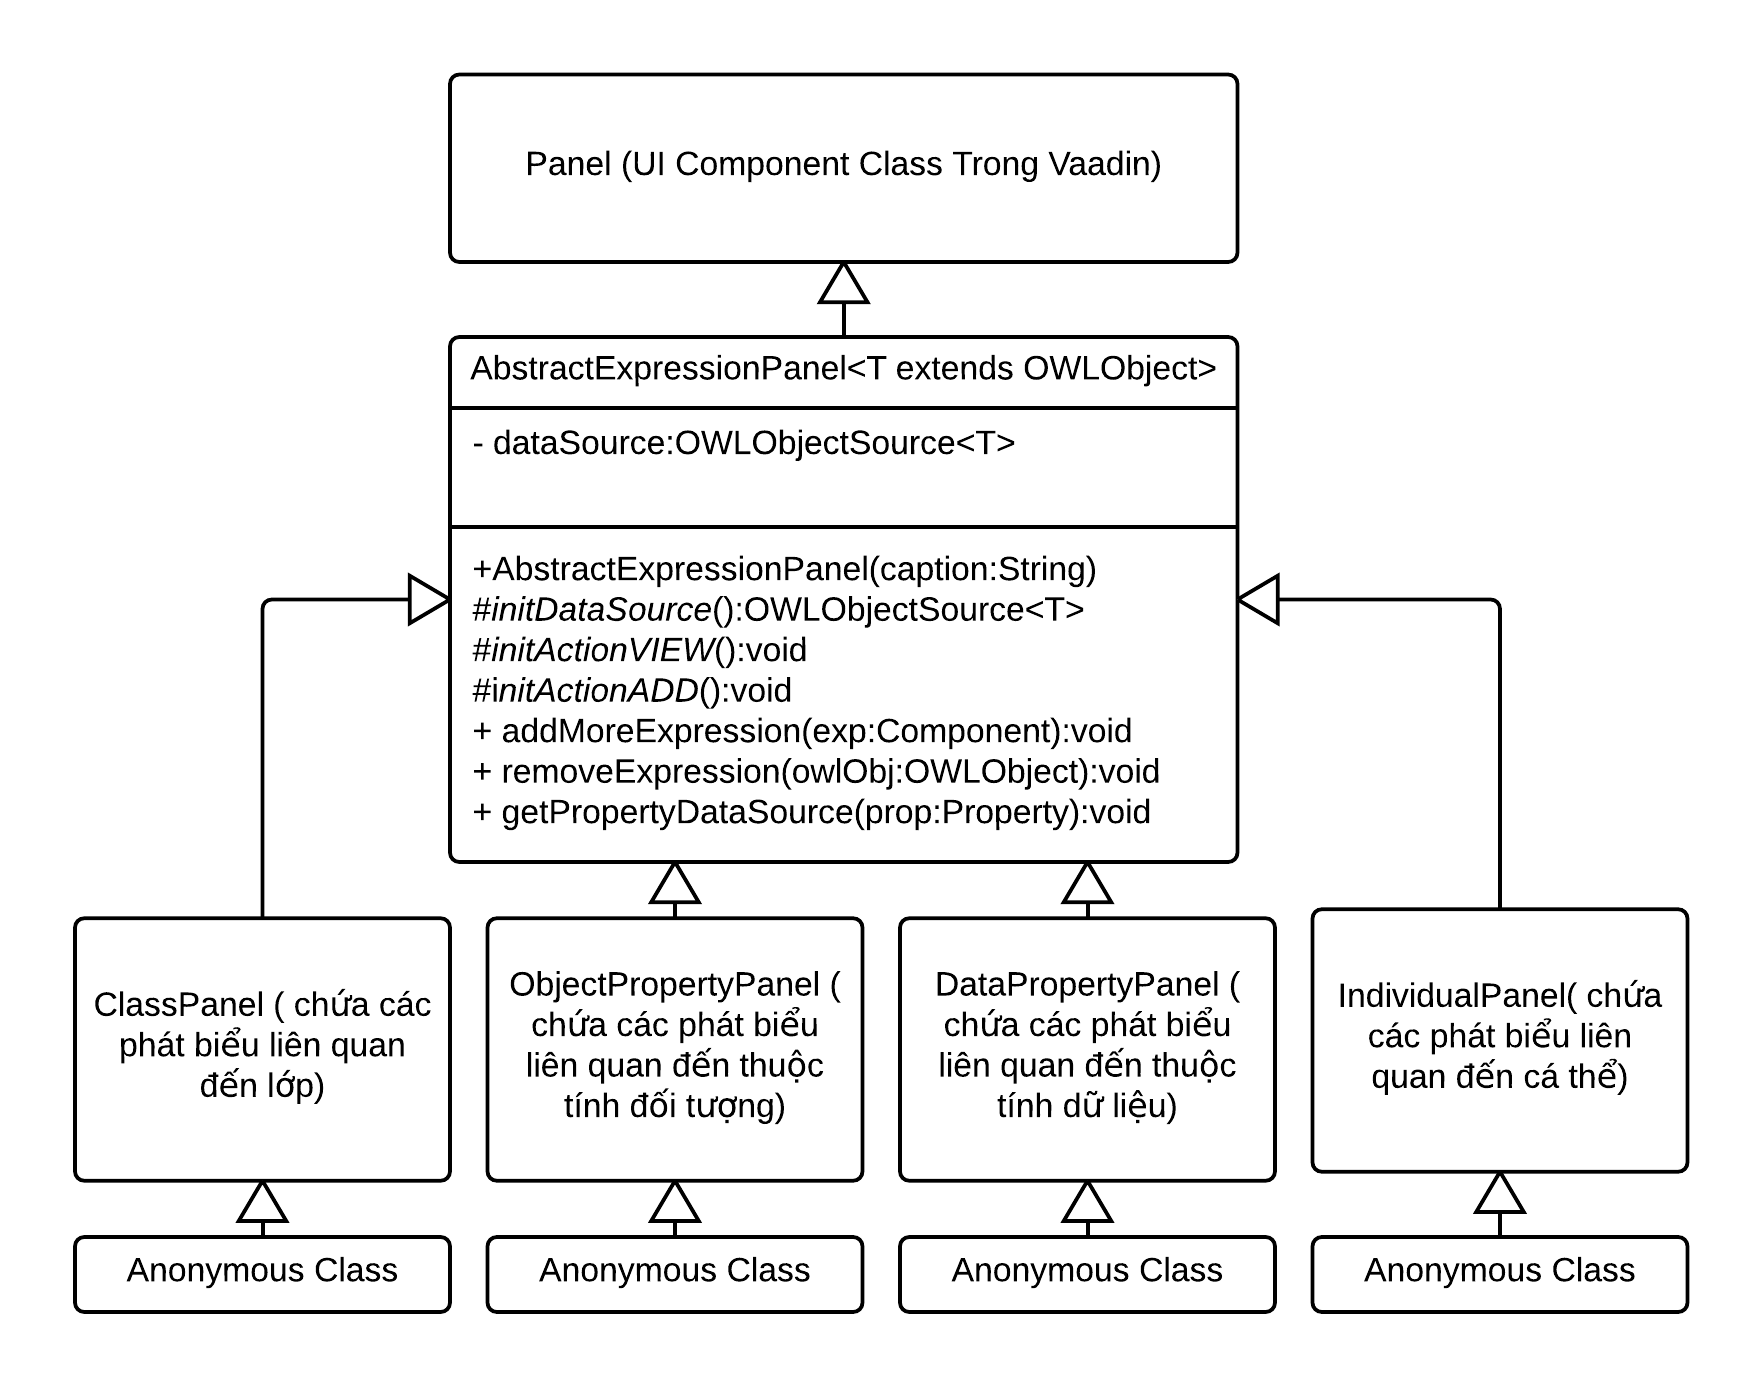
\includegraphics[width=155mm]{Figures/uml_owleditor_abstractpanel_nobackground.png}
	\caption{Class Diagram của AbstractExpressionPanel\label{overflow}}
\end{figure}
Như chúng ta sẽ thấy trong sơ đồ ở hình 4.7 thì tất cả các panel mô tả các phát biểu đều được kế thừa từ đây. Các phương thức in nghiêng trong lớp abstract này chính là các phương thức abstract sẽ được xây dựng cụ thể ở những lớp con của chúng để phù hợp với phát biểu mà chúng muốn diễn tả. Ví dụ chúng em, muốn diễn ta một phát biểu về về lớp con (SubClassOf), thì sẽ khai báo một Anonymous Class từ ClassPanel như sau:
\begin{itemize}
\item initActionADD
\begin{verbatim}
// định nghĩa cụ thể là phải tạo event SubClass
UI.getCurrent().addWindow(new buildAddClassExpressionWindow(
  expression -> eKit.getDataFactory().getSubClassOfAddEvent(...))
);
\end{verbatim}
\item initActionVIEW
\begin{verbatim}
//: định nghĩa cụ thể là phải tìm hiển thị các lớp cha của
Collection<OWLClassExpression> ces = 
            EntitySearcher.getSuperClasses(..);
// tạo các Label trên panel
ces.forEach(ce -> panel.addComponent(new ClassLabel(ce, ...)));
// Nếu trạng thái reasoner bật thì lấy các thông tin về lớp cha
Set<OWLClass> clzz = editorKit.getReasoner().getSuperClasses(...)
// Tạo các label tô đậm trên panel 
clzz.forEach(c -> panel.addComponent(new InferredLabel(c)));
\end{verbatim}
\end{itemize}
\begin{figure}[h!]
	\centering
	\frame{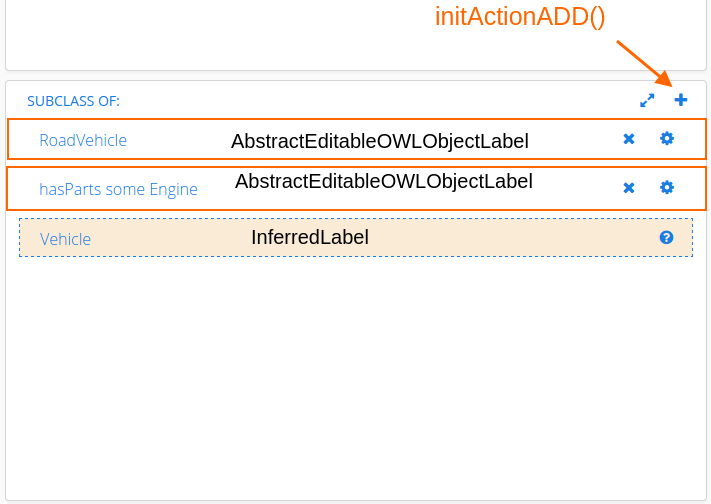
\includegraphics[width=120mm]{Figures/owleditor_expressionpanel.png}}
	\caption{Panel mô tả các phát biểu SubClassOf\label{overflow}}
\end{figure}
Khi chọn biểu tượng dấu "+" hoặc bánh răng biểu như trong hình 4.8, sẽ mở ra một cửa sổ mới để chúng ta có thể biên tập các mô tả lớp (ClassExpression) hoặc một cửa sổ để chỉnh sửa các phát biểu này, các loại cửa sổ này đều được xây dựng từ một lớp Abstract là AbstractOWLExpressionEditorWindow.
\subsubsection{AbstractOWLExpressionEditorWindow}
\begin{figure}[h!]
	\centering
	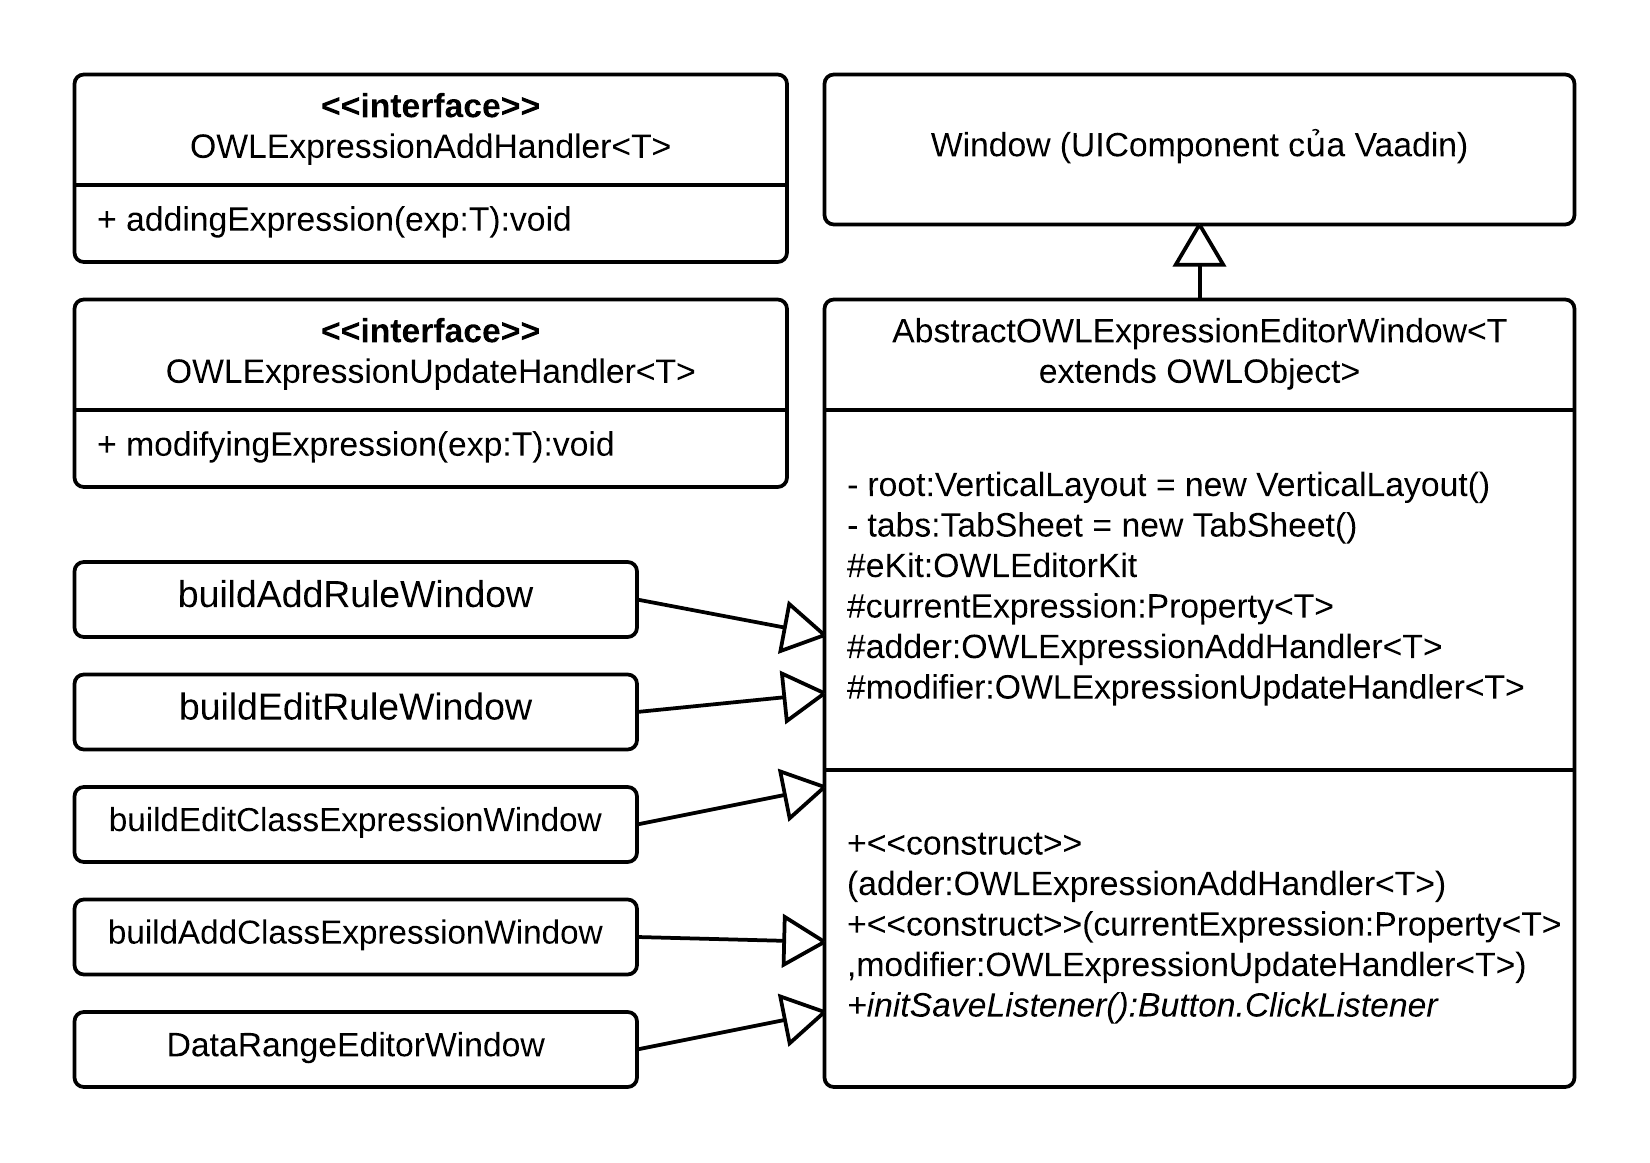
\includegraphics[width=155mm,height=100mm]{Figures/uml_owledtior_abtractwindow.png}
	\caption{Class Diagram của AbstractOWLExpressionEditorWindow\label{overflow}}
\end{figure}
Trong hình 4.9 tập hợp hết tất cả các lớp con là các cửa sổ dùng để thêm hoặc sửa mô tả lớp, kiểu dữ liệu trong hệ thống, chúng đều được mở rộng từ abstract này. Đáng chú ý chúng em cũng đang viết các interface dùng trả về các sự kiện phù hợp với từng loại phát biểu (cách hoạt động của chúng như đã trình bày trong mục 4.3.1.2). Một điểm không được thể hiện trong sơ đồ lớp đó chính là việc sử dụng EventBus trong đây. EventBus được sử dụng trong phương thức \textit{initSaveListener}. Ví dụ để cài đặt một event chỉnh sửa một mô tả lớp, chúng ta sẽ đưa đoạn code sau vào initSaveListener.
\begin{verbatim}
OWLClassExpression ce = editorKit.parseClassExpression(editor.getValue());
OWLEditorEventBus.post(modifyExpression.modifyingExpression(ce));
\end{verbatim}
\begin{figure}[h!]
	\centering
	\frame{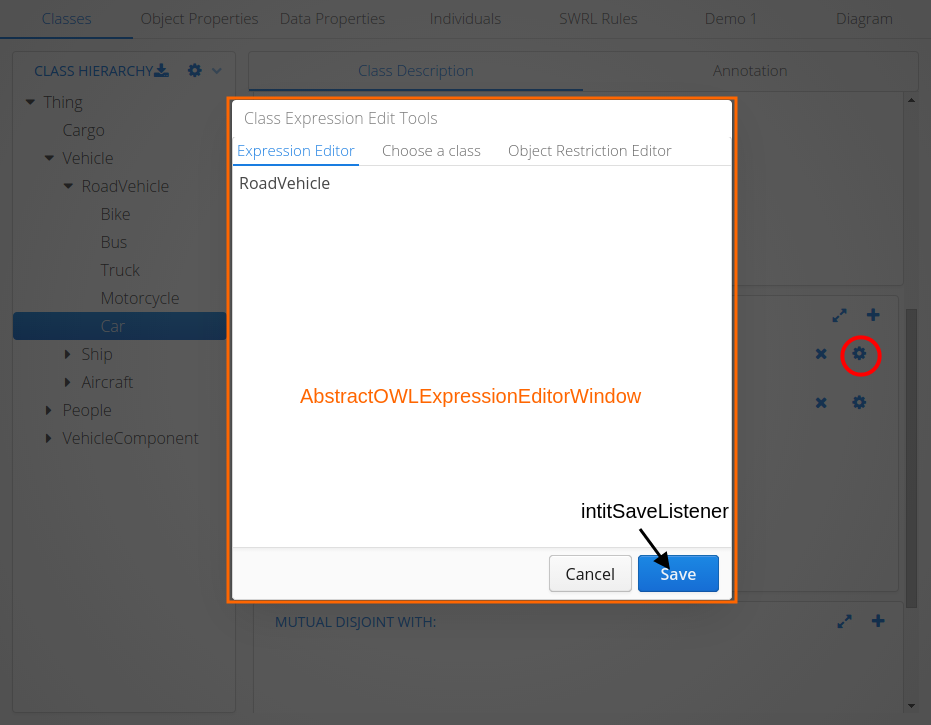
\includegraphics[width=155mm]{Figures/owleditor_ceeditor.png}}
	\caption{Biên tập và chỉnh sửa mô tả lớp\label{overflow}}
\end{figure}
Biến \textit{modifyExpression} là một interface \textit{OWLExpressionUpdateHandler} (Hình 4.9).  Interface này sẽ được định nghĩa thông qua một lớp gọi là \textit{AbstractEditableOWLObjectLabel} (Hình 4.8), Label được thêm vào panel trong \textit{initActionVIEW} ở mục trên, ClassLabel cũng chính là một \textit{AbstractEditableOWLObjectLabel}. Vì thế nếu nhìn chi tiết hơn vào đoạn code ở trên ta có ClassLabel được tạo ra như sau:
\begin{verbatim}
... = new ClassLabel(new OWLClassExpressionSource(ce),
() -> eKit.getDataFactory().getSubClassOfRemoveEvent(currentCls, ce),
newClsEx -> eKit.getDataFactory()
         .getSubClassOfModEvent(currentCls, newClsEx, currentClsEx))
\end{verbatim}
Bởi vì chỉ khi tạo một panel cụ thể cho một phát biểu chúng ta mới biết đó là loại sự kiện gì cho nhóm phát biểu nào (lớp, thuộc hay cá thể). Như đã nói việc xây dựng những interface tiện ích như trên giúp chúng em tiết kiệm rất nhiều công sức khi thực hiện. Trở lại với cửa sổ của biên tập mô tả lớp vừa rồi, khi nhấn "Save" sự kiện sẽ được công bố lên EventBus. Vậy đâu mới là đối tượng tiếp nhận sự kiện vừa rồi. Đó là thành phần sẽ được giới thiệu ngay sau đây.
\subsubsection{AbstractPanelContainer}
Xem lại hình 4.3, đây là thành phần chứa tất cả các \textit{AbstractExpressionPanel} và đặc biệt đây là thành phần chứa 3 loại Subscriber tương ứng với 3 loại sự kiện là thêm, xóa và sửa. Lấy ClassExpressionPanelContainer (lớp kế thừa từ lớp abstract này) làm ví dụ, nó sẽ có 3 subscriber như sau:
\begin{verbatim}
@Subscribe public void afterClassAxiomAdded(ClassAxiomAdded event) 
@Subscribe public void afterClassAxiomRemoved(ClassAxiomRemoved event) 
@Subscribe public void afterClassAxiomModified(ClassAxiomModified event)
\end{verbatim}
Các thay đổi sẽ được áp dụng trực tiếp vào ontology thông qua:
\begin{verbatim}
@Subscribe public void afterClassAxiomAdded(ClassAxiomAdded e) {
  ChangeApplied ok = eKit.getModelManager()
	.applyChange(new AddAxiom(eKit.getActiveOntology(), e.getAxiom()));
  if(ok == SUCCESSFULLY) {
  e.getAxiom().accept(addHelper(e.getAxiom(), e.getOwner())); }
} 
\end{verbatim}
Sau khi các thay đổi được áp dụng thành công, chúng sẽ được cập nhật lên ontology bằng addHelper/removeHelper, cả hai đối tượng này đêu là \textit{OWLAxiomVisitor} được cài đặt thông qua \textit{OWLAxiomVisitorAdapter} để truy vấn đến những thay đổi có liên quan đến phát biểu có trong sự kiện. Ví dụ: nếu các phát biểu đó liên quan đến lớp thì chúng ta chỉ định nghĩa lại giải thuật cho các phương thức visit(OWLClassAssertionAxiom/ OWLDisjointClassesAxiom/ OWLEquivalentClassesAxiom/ OWLSubClassOfAxiom ) trong adapter.
\subsubsection{SWRL Rule Tab}
Tab này có đặt điểm khác sao với các tab còn lại, chỉ gồm một thành phần chính là một Table chứa các SWRL trong tài liệu OWL 2 Ontology. Khi right-click sẽ có các chức năng thêm/xóa/sửa rule được chọn.
\begin{figure}[h!]
	\centering
	\frame{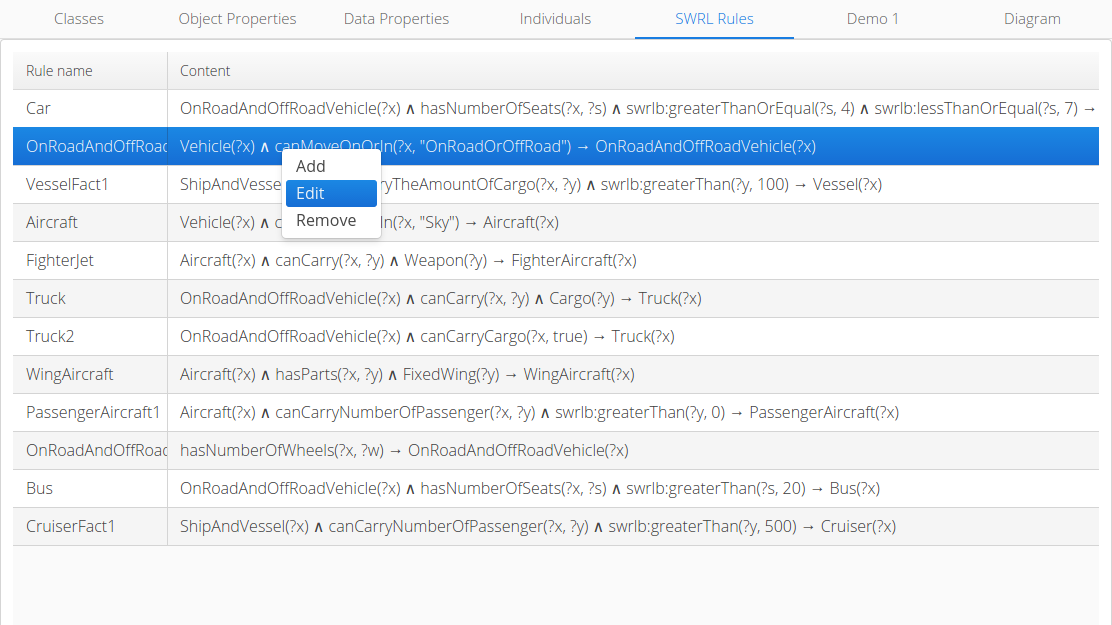
\includegraphics[width=155mm]{Figures/owleditor_swrlSheet.png}}
	\caption{SWRL Rule Tab\label{overflow}}
\end{figure}
Khi chọn thêm hay sửa rule, sẽ hiện ra một cửa sổ để thêm hoặc chỉnh sửa, về cách thức tổ chức sự kiện thì tương tự với \textit{AbstractOWLExpressionEditorWindow} vì chúng được kế thừa từ lớp Abstract này (Hình 4.9). Duy chỉ có một khác biệt đó là thay vì có một \textit{AbstractPanelContainer} để chứa các Subscriber (phục vụ các sự kiện thêm, xóa, sửa rule) thì các Subscriber nằm trong chính \textit{RuleSheet} - layout chính của tab này.
\begin{figure}[h!]
	\centering
	\frame{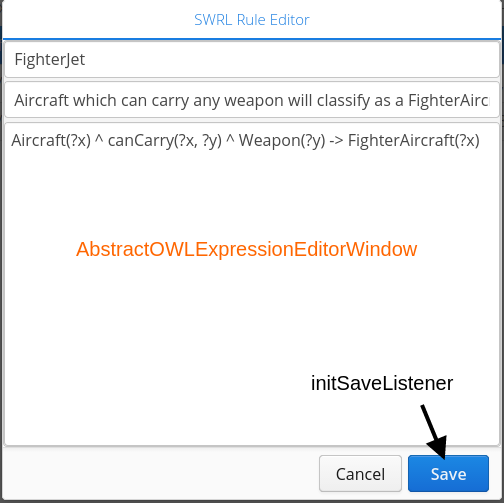
\includegraphics[width=100mm]{Figures/owleditor_ruleeditor.png}}
	\caption{Cửa sổ biên tập SWRL Rule\label{overflow}}
\end{figure}
\paragraph{Kết luận} Tất cả các thành phần vừa được chúng em vừa giới thiệu, đều được sử dụng để mở rộng thành những thành phần giao diện cụ thể trong ứng dụng. Với số 4 loại thực thể (lớp, thuộc tính đối tượng/dữ liệu và cá thể) và rất nhiều dạng phát biểu (Axiom), chúng em nghĩ việc xây dựng các thành phần giao diện thành các lớp Abstract, sử dụng interface để làm các action handler hoặc xây dựng dữ liệu theo tính đa hình đã phát huy hiệu quả rất lớn là chúng em đã tách biệt thành phần giao diện và dữ liệu (thực thể, phát biểu) với nhau, nhằm tránh việc xây dựng lại từng giao diện cho từng phát biểu, thực thể.
\section{Hiện thực khả năng phân loại tự động của ontology đã thiết kế}
Đây chính là mục tiêu cuối cùng mà cả hệt thông muốn hướng tới, chứng minh tính khả thi trong việc sử dụng ontology để phân loại. Ontology transport \cite{owleditorSrc} được xây dựng giống như thiết kế ở chương 3. Chúng em sẽ thực nghiệm việc suy luận (reasoning) qua đó phân loại các cá thể thuộc lớp \textit{Vehicle} vào trong các lớp con của nó.
\begin{figure}[h!]
	\centering
	\frame{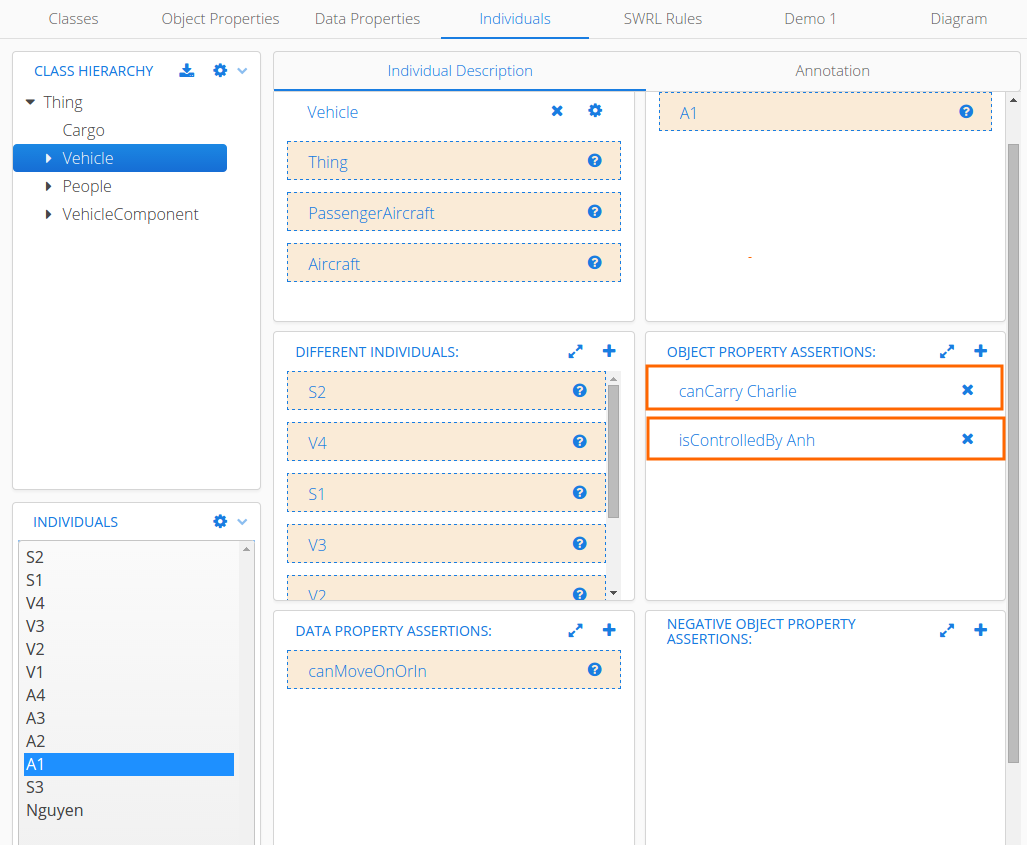
\includegraphics[width=155mm]{Figures/classify1.png}}
	\caption{Phân loại dựa vào các phát biểu tương đương\label{overflow}}
\end{figure}
\subsection{Phân loại dựa vào các phát biểu tương đương} 
Cá thể A1 thuộc các lớp Aircraft (Hình 4.13), chọn dấu chấm ? trên phát biểu chúng ta sẽ nhận được giải thích sau:
\begin{verbatim}
Aircraft EquivalentTo Vehicle and (isControlledBy some Pilot)
Anh Type Pilot
A1 isControlledBy Anh
A1 Type Vehicle
\end{verbatim}
Trong mọi loại phát biểu thì phát biểu tương đương Equivalent là loại phát biểu có ràng buộc lớn nhất giữa các lớp với nhau, nghĩa là một cá thể hội đủ điều kiện của \textit{Vehicle} \textbf{và} \textit{(isControlledBy some Pilot)} sẽ thuộc loại \textit{Aircraft}. Do A1 đã thuộc \textit{Aircraft} do các phát biểu trên nên nó cũng thuộc \textit{PassengerAircraft} dựa theo các phát biểu sau
 \begin{verbatim}
PassengerAircraft EquivalentTo Aircraft and (canCarry some Passenger)
Charlie Type Passenger
A1 canCarry Charlie
\end{verbatim}
\begin{figure}[h!]
	\centering
	\frame{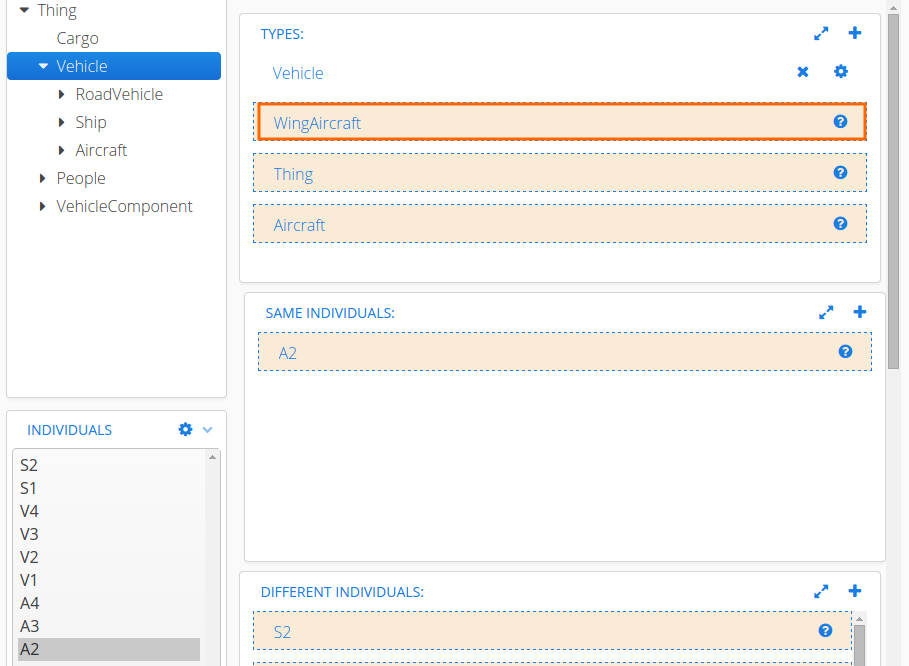
\includegraphics[width=145mm]{Figures/classify2.png}}
	\caption{Phân loại dựa trên Domain của thuộc tính đối tượnglabel{overflow}}
\end{figure}
\subsection{Phân loại dựa trên Domain của thuộc tính đối tượng} 
Chọn vào dấu ? để xem giải thích (Hình 4.14, chúng ta sẽ nhận được các giải thích sau cho lý dó \textit{A2} là \textit{WingAircraft}
\begin{verbatim}
hasWing Domain WingAircraft
A2 hasWing XWing
\end{verbatim}
Giải thích chỉ có những cá thể thuộc lớp \textit{WingAircraft} mới có thuộc tính đối tượng \textit{hasWing}, mà A2 \textit{hasWing} XWing (không cần biết XWing thuộc lớp nào) nên A2 cũng thuộc \textit{WingAircraft}.
\subsection{Phân loại theo SWRL Rule và thuộc tính dữ liệu} 
Cá thể V4 đã thuộc lớp \textit{RoadVehicle} trước, khi phân loại chúng ta thấy nó sẽ thuộc vào lớp \textit{Bus}, đây là lý do \begin{verbatim}
RoadVehicle(?x) ^ hasNumberOfSeats(?x, ?s) 
               ^ swrlb:greaterThan(?s, 20) -> Bus(?x)
V4 hasNumberOfSeats 21
V4 Type RoadVehicle
\end{verbatim}
\textit{V4} được khai báo là Vehicle có thuộc tính dữ liệu \textit{hasNumberOfSeats} (có số chỗ ngồi) với giá trị 21, mà SWRL Rule nói rằng phương tiện đường bộ nào có số chỗ ngồi lớn hơn hoặc bằng 20 đều là xe Bus (Hình 4.15).
\begin{figure}[h!]
	\centering
	\frame{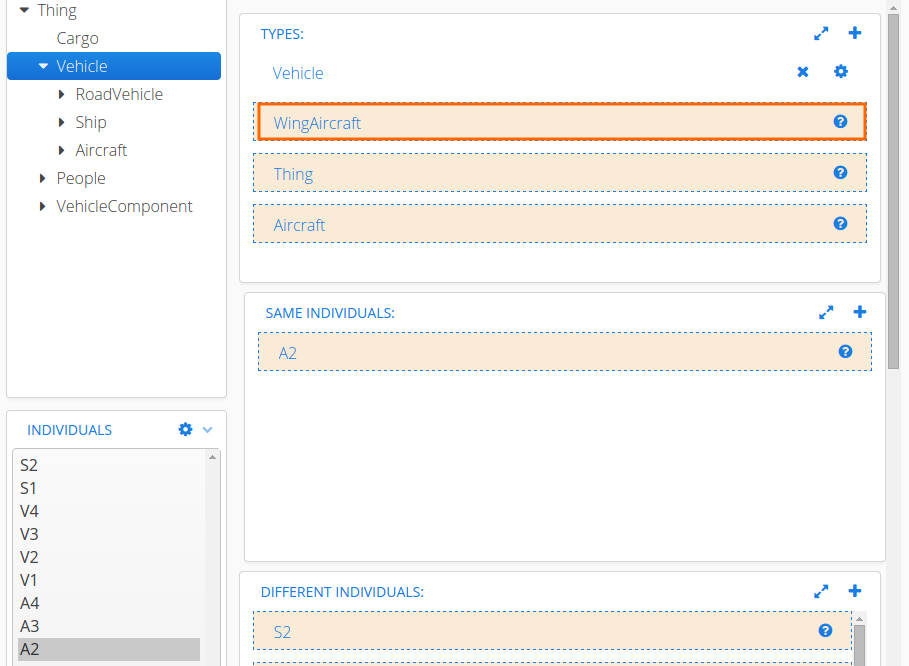
\includegraphics[width=145mm]{Figures/classify2.png}}
	\caption{Phân loại dựa trên Domain của thuộc tính đối tượnglabel{overflow}}
\end{figure}
Trên đây, là 3 ví dụ khá đơn giản về cách sử dụng các phát biểu của riêng OWL 2 hay sử dụng chúng kết hợp chúng với SWRL Rule để phân loại. Trên thực tế sẽ có những trườgn hợp phức tạp hơn, ví dụ của chúng em chỉ muốn kiểm chứng tính khả thi và khả năng của OWL 2 và SWRL.
\section{Tính năng hỗ trợ phân loại - Demo Tab}
\begin{figure}[ht!]
	\centering
	\frame{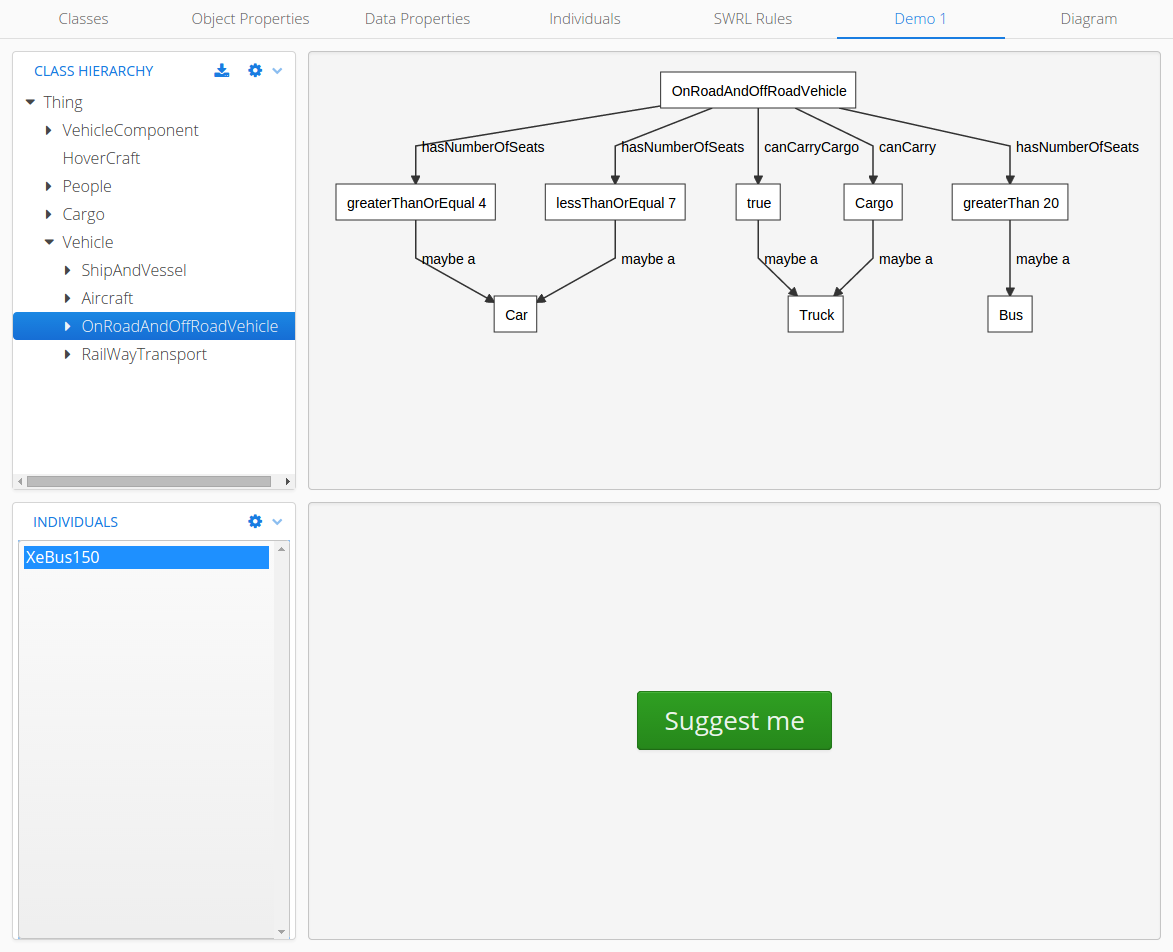
\includegraphics[width=145mm]{Figures/owleditor_demo1.png}}
	\caption{Tính năng hỗ trợ phân loại Demo Tab (phần 1)\label{overflow}}
\end{figure}
Việc sử dụng SWRL Rule hay đơn giản hơn là đọc và hiểu ý nghĩa có nó thường rất khó đối với người dùng thông thường, chưa kể đến việc chưa có cơ chế tổ chức các SWRL rule một cách khoa học, sẽ có những trường hợp chúng ta vô tình tạo ra những điều kiện trùng nhau dẫn đến 2 kết quả khác nhau hoặc ngược lại. Hiểu được nhược điểm này của SWRL Rule, chúng em đã thiết kế thêm tính năng hỗ trợ phân loại với giao diện là Tab Demo trong ứng dụng, với khả năng vẽ ra một sơ đồ dựa theo chuỗi các điều kiện - kết quả có liên quan đến lớp đang chứa cá thể được chọn để phân loại. Để minh họa cho tính năng này ,chúng em xin trích một đoạn chứa các SWRLRule trong ontology \textit{Transport.owl} \cite{owleditorSrc} (được chúng em xây dựng để làm demo cho tính năng phân loại). Hình trên mô tả lại các rule sau:
\begin{verbatim}
# Phương tiện đường bộ có thể chở hàng hóa (Cargo) là xe tải (Truck)
OnRoadAndOffRoadVehicle(?x) ^ canCarry(?x, ?y) ^ Cargo(?y)  -> Truck(?x)
# Phương tiện đường bộ có khả năng chở hàng là xe tải (Truck)
OnRoadAndOffRoadVehicle(?x) ^ canCarryCargo(?x, true) -> Truck(?x)
# Phương tiện đường bộ có số 4 <= chỗ ngồi <= 7 là xe hơi (Car)
OnRoadAndOffRoadVehicle(?x) ^ hasNumberOfSeats(?x, ?s)
^ swrlb:greaterThanOrEqual(?s, 4) 
^ swrlb:lessThanOrEqual(?s, 7)  -> Car(?x)
# Phương tiện đường bộ có số chỗ ngồi >= 20 là xe Bus 
OnRoadAndOffRoadVehicle(?x) ^ hasNumberOfSeats(?x, ?s) 
^ swrlb:greaterThan(?s,20) -> Bus(?x)                               
\end{verbatim}
Trong hình chỉ miêu tả những rule nào có liên quan đến lớp \textit{OnRoadAndOffRoadVehicle} vốn là lớp chứa cá thể \textit{XeBus150} trong hình, làm vậy để hạn chế những thông tin không cần thiết đối với người dùng. Khi chọn \textit{Suggest Me} sẽ tạo ra một loại các UI Component phục vụ để tạo ra các phát biểu về cá thể \textit{XeBus150}.
\begin{figure}[h!]
	\centering
	\frame{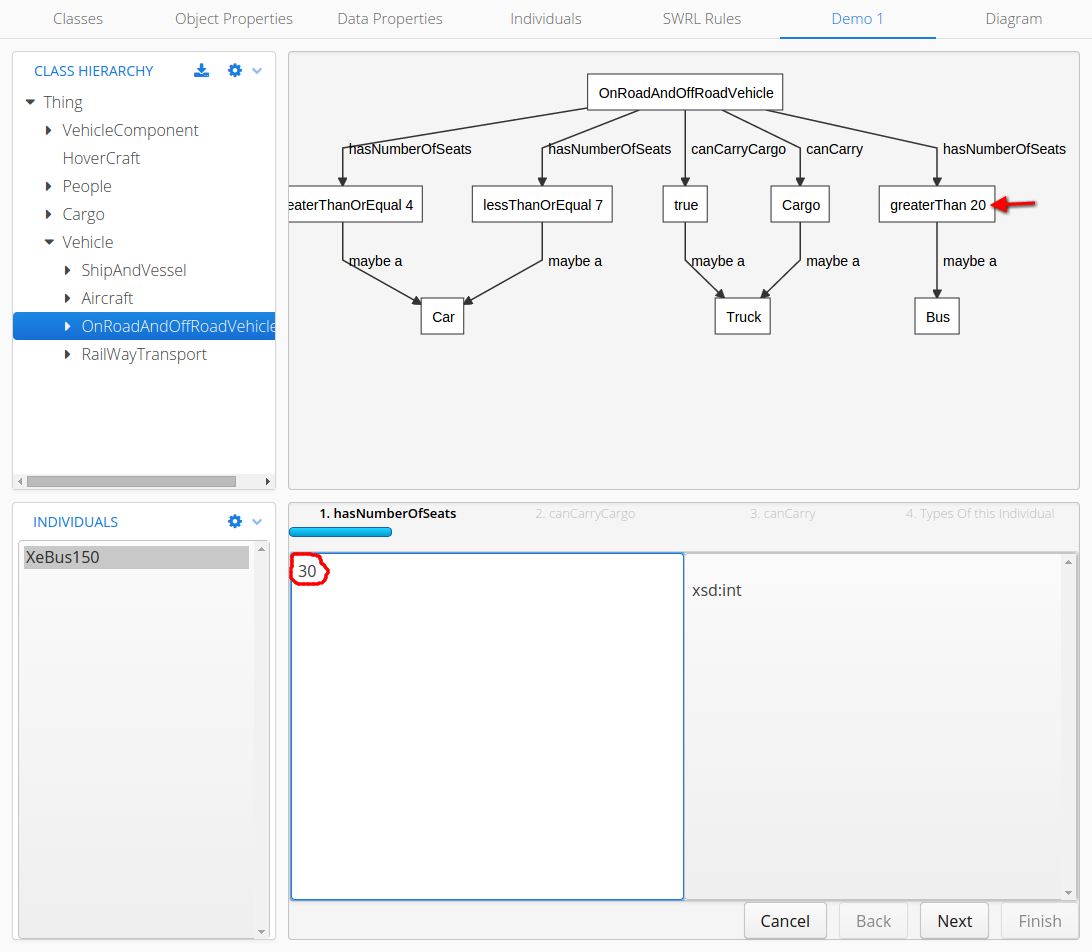
\includegraphics[width=145mm]{Figures/owleditor_demo2.png}}
	\caption{Tính năng hỗ trợ phân loại Demo Tab (phần 2)\label{overflow}}
\end{figure}
\begin{figure}[h!]
	\centering
	\frame{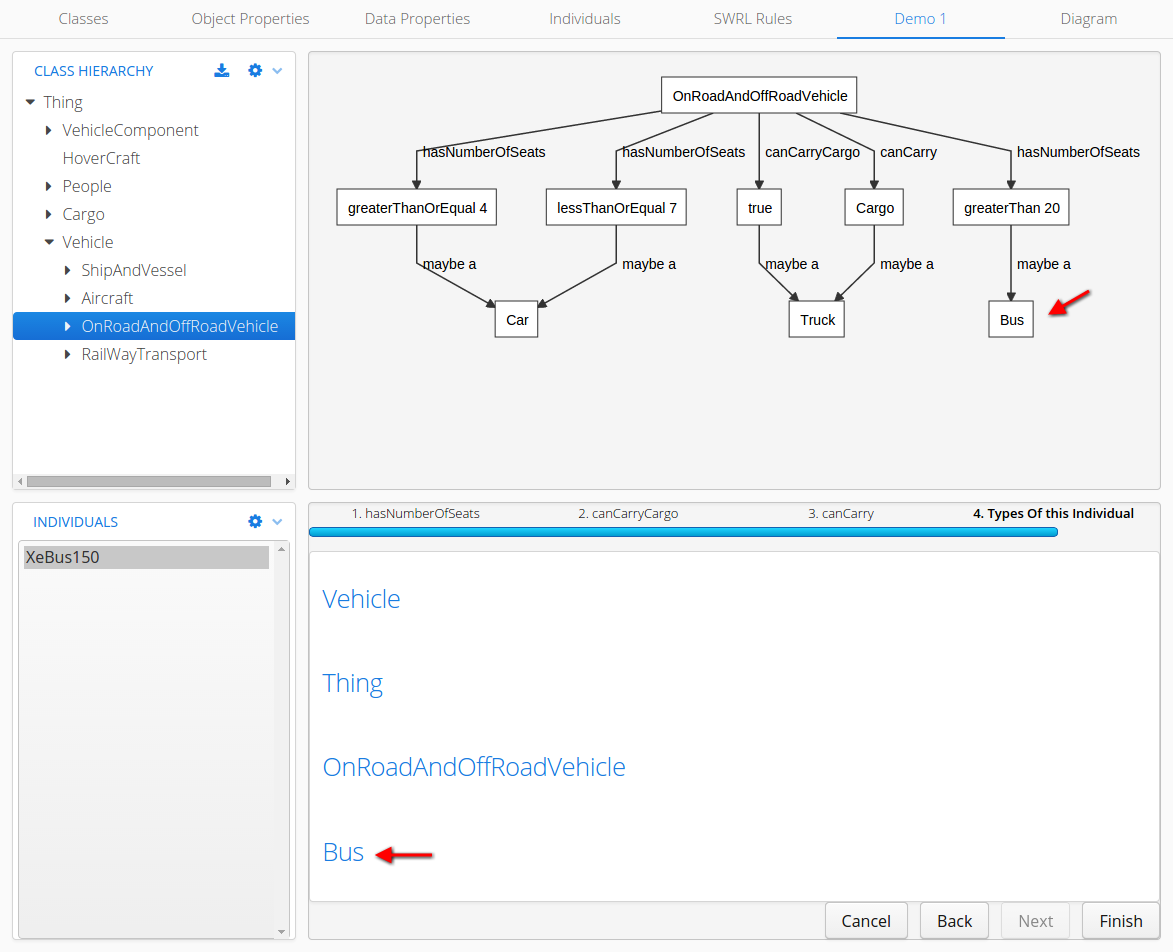
\includegraphics[width=145mm]{Figures/owleditor_demo3.png}}
	\caption{Tính năng hỗ trợ phân loại Demo Tab (phần 3)\label{overflow}}
\end{figure}
Trong hình trên mỗi bước tương ứng với những phát biểu có liên quan đến \textit{OnRoadAndOffRoadVehicle} như trong sơ đồ. Miền dữ liệu (Range) của thuộc tính dữ liệu và thuộc tính đối tượng cũng sẽ được áp dụng nhằm giảm bớt những thông tin không cần thiết, thuộc tính \textit{hasNumberOfSeats} có DataPropertyRange( xsd:int) nên ở cột bên phải chúng ta chỉ thấy kiểu dữ liệu này thay vì là một loạt kiểu dữ liệu như xsd:string, xsd:byte, v.v... . Khi đến bước cuối cùng, reasoner sẽ đánh giá lại các thông tin mà chúng ta vừa nhập vào ở các bước trước để đưa kết quả phân loại phù hợp như đã được biểu diễn trong sơ đồ.